%\documentclass[letterpaper, 10pt]{sigcomm-alternate}

\documentclass[peerreview, a4paper, 7pt]{IEEEtran}
%\documentclass[a4paper, 10pt]{IEEEtran}
%\documentclass[a4paper]{scrreprt}
%\documentclass[a4paper,headlines=2.1]{scrartcl}
%\documentclass[a4paper,BCOR12mm,DIVcalc,twoside]{scrartcl}
\usepackage{bookman}
\usepackage{times}
\usepackage{graphicx}

\usepackage[hidelinks]{hyperref}
%\typearea[12mm]{1}% entspricht obigen Optionen

%\renewcommand*{\titlepagestyle}{empty}



\title{Web Cryptography: \\Supporting the FIDO Protocol Family\thanks{Position paper for the 'W3C Workshop on Authentication, Hardware Tokens and Beyond', 10-11 September 2014, Silicon Valley (Mountain View), California. This paper represents the views of the author.}}


\author{Hannes Tschofenig\\\textit{\href{mailto:hannes.tschofenig@arm.com}{hannes.tschofenig@arm.com}}}
\date{July 25, 2014}

\begin{document}
\maketitle


\begin{abstract}

The last few years have been quite disturbing from a Web security point of view: a number of high-profile security incidents have gotten a lot
of press attention but various various projects, such as the National Strategy for Trusted Identities in Cyberspace (NSTIC) in the US and the 
European STORK project, had been launched to improve the Web authentication and identity eco-system. Among the security community there is 
consensus that Internet and Web security could be improved by reducing the use of low-entropy passwords and that the deployment of other 
types of credentials has to be improved. \\

FIDO (Fast IDentity Online) is the most recent attempt to reduce reliance on passwords and complements efforts to increase the deployment of 
identity management infrastructures, such as those offered by OpenID Connect. In this position paper the author provides a high-level 
introduction to FIDO, discusses interoperability needs, and makes a few recommendations for work in the W3C. 

\end{abstract}

\section{FIDO Overview}

The FIDO (Fast IDentity Online) Alliance~\cite{fido} is developing two protocols, namely the Universal Authentication Framework (UAF)~\cite{uaf} and the Universal Second Factor (U2F)~\cite{u2f}, with the aim to improve authentication on the Web. U2F aims to introduce another factor to password-based authentication and therefore does not aim to get rid of passwords. UAF, on the other hand, makes use of local authentication, such as using biometrics, and allows password-free authentication. From an architecture point of view both protocols operate very similar\footnote{For historical reasons the two protocols use different terminolgy and have a different on the wire representation. U2F calls the hardware-based key store 'U2F Token' whereas UAF refers to it as the 'Authenticator'. In this paper we use the term 'Authenticator' to refer to both of them. Note also that the FIDO U2F/UAF specifications use the term 'Relying Party' to refer to the Web server-side entity. Other publications often use the term 'Identity Providers' instead.}: users make use a hardware-based key store, the Authenticator, that executes an authentication protocol with a Web server using a browser, or a native application as a relay. 

The main parties are shown in Figure~\ref{fido-overview-figure}. This new authentication and key exchange protocol uses public key cryptography and nonces for authentication of the Authenticator to the Relying Party. Demonstrating possession of the private key via the Authenticator is only useful if the corresponding public key is registered with the server, which happens during an initial registration step. Server-side authentication, via Transport Layer Security (TLS), is essential during this step to ensure that the public key is registered with the intended origin. To avoid privacy problems an Authenticator maintains different public keys with different origins: sharing public keys with different origins allows Relying Parties to correlate transactions. 

\begin{figure}[!htbp]
 \centering
 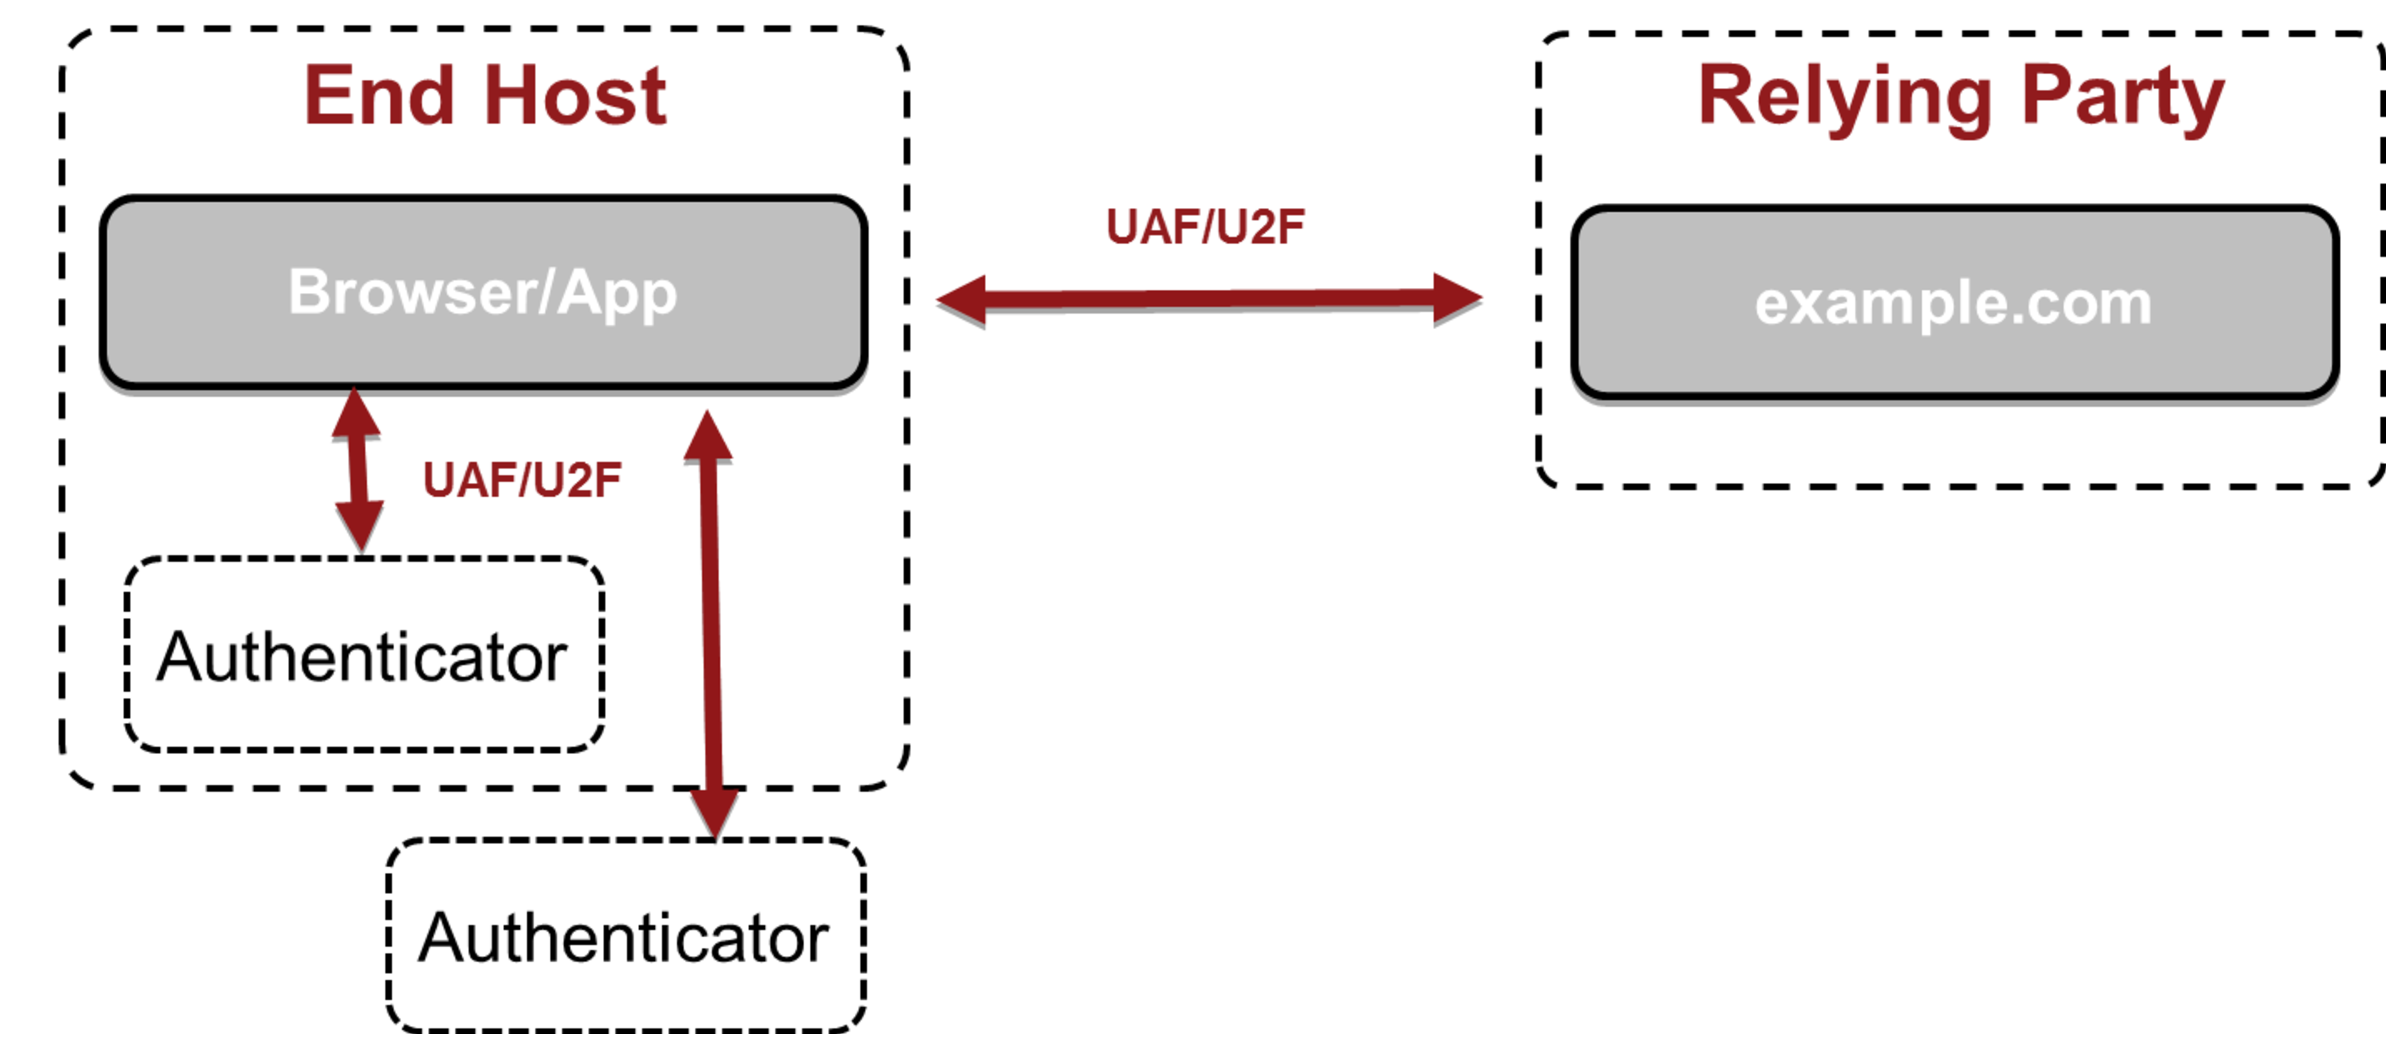
\includegraphics[scale=0.30]{architecture.eps}
 \caption{FIDO: High-Level Overview.}
\label{fido-overview-figure}
\end{figure}

Figure~\ref{fido-overview-figure} also aims to illustrate that the Authenticator may be located outside the end device. For example, the Authenticator may be connected to the end host via a USB interface (i.e., the Authenticator is a USB-based token.) or connected to the end host using some radio technology, such as Bluetooth Smart. In other cases, the end host might itself have a trusted execution environment, as it is increasingly common with laptops and smart phones. Standardizing the communication with the Authenticator is only important if users are unwilling to install software for individual Authenticators. For Bluetooth Smart-based devices, however, users today often have to install apps of the vendor and hence it remains to be seen whether this changed user expectation simplies the introduction and deployment of new Authenticators. 
 
\section{Interoperability}

Changing the state of online authentication on the Web has been challenging since various parties need to cooperate to reach widespread deployment, as Figure~\ref{fido-overview-figure} shows. Designing new authentication protocols (from a purely technical point of view) is relatively easy, as the number of proposed solutions illustrates. Relying Parties rarely have incentives to deploy a new authentication mechanism since those mechanisms are not supported by browsers, desktop/laptop operating systems, nor by smart phone apps. Developing solutions and distributing the necessary devices has been costly for companies (such as financial institutions). A main goal of any standardization effort is therefore to lower the barrier for Relying Parties. Browser and operator system vendors have been reluctant to support any authentication technology beyond their own development. This has been the status so far and the reason for a number of failed attempts in this space. 

Several environtal factors have changed in the meanwhile that give reasons for hope, such as 
\begin{itemize}
  \item Increasing number of security incidents increase awareness and put pressure on various parties. 
  
  \item Many applications are now browser-based and the update cycle of browsers has increased substantially. This allows a faster roll-out of new functionality. Smart phone apps also have excellent software update capabilities. 
  
  \item The increasing deployment of smart phone and tablets has lead to a new user behavior and user expectations. These devices also increase the need to search for better usability of authentication mechanisms. High-entrophy passwords tend to be challenging to memorize and to enter. 
  
  \item The W3C Web Crypto API offers a flexible new way to develop new authentication protocols using JavaScript and browser vendors seem to be feel comfortable with this new mechanism (although it is still a bit early to tell how successful the mechanism will be).
  
  \item An increasing number of identity providers have been deployed and many identity federations (using OAuth/OpenID Connect and SAML) are in use. The use of identity federations simplifies deployment of authentication technologies since new authentication mechanisms have to be enabled only at identity providers rather than at each relying party. This lowers the cost of deployment, which is one of the arguments for using identity federations. The use of identity federations will be crucial for the success of any online Web authentication mechanism. 
  
\end{itemize} 


\begin{figure}[!htbp]
 \centering
 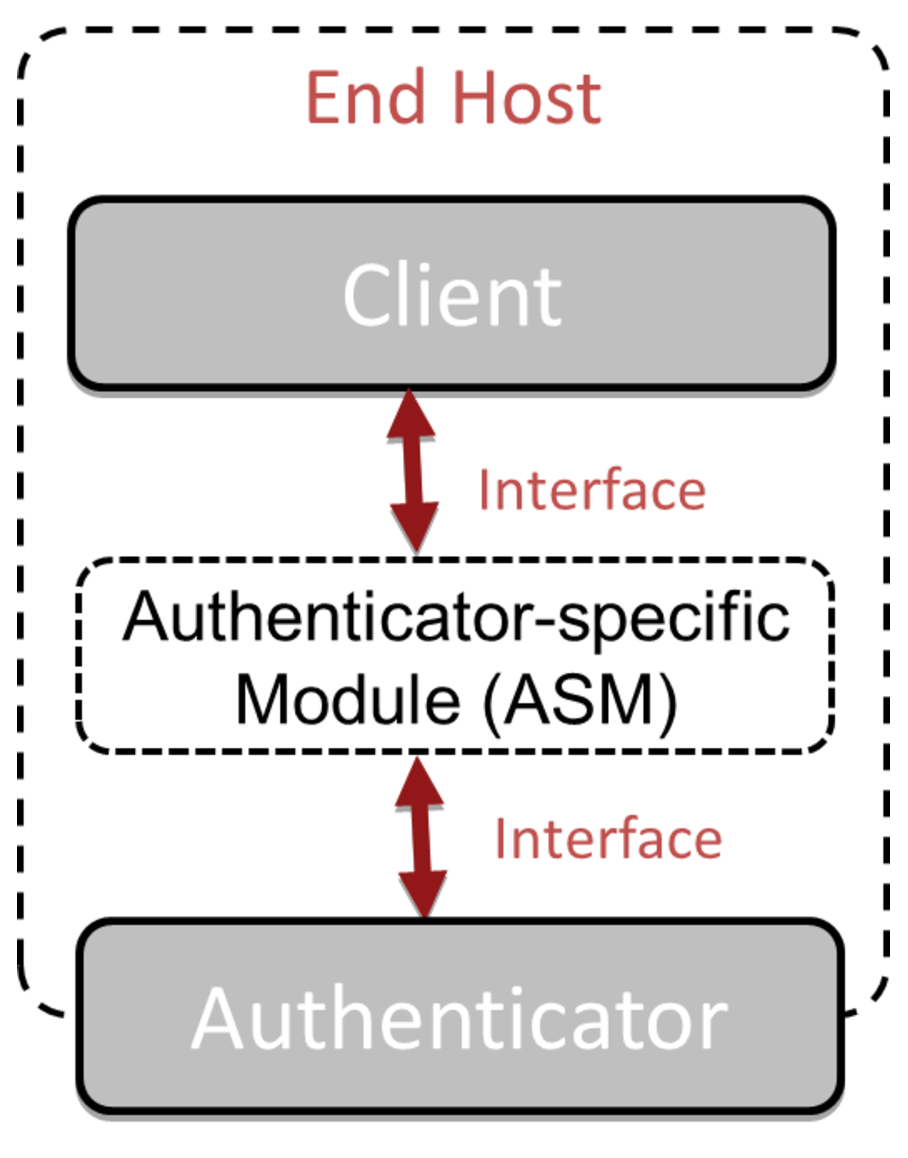
\includegraphics[scale=0.30]{asm.eps}
 \caption{FIDO: Client-Side Abstraction.}
 \label{asm-figure}
\end{figure}

Assuming widespread adoption of the W3C Crypto API might therefore lead to the premature impression that the online authentication topic is now solved since the FIDO protocols could be implemented using this JavaScript-based API. Unfortunately, this is not the case for the following reasons:
\begin{itemize}
  \item The UAF protocol requires the browser to query the list of available Authenticators and their capabilities. This information, when passed on to the Relying Party, allows policy decisions to be made: the quality of authentication varies with Authenticators and Relying Parties may accept some Authenticators but not others.
 
  \item The UAF and the U2F protocols assume the use of a hardware-based key store and even multiple of those may be available at a given host. Consequently, there has to be a way for selecting the appropriate Authenticator. 
  
  \item Finally, the browser or the application has to interact with the Authenticator through an intermediate layer of abstraction, the Authenticator-specific Module (ASM). The ASM allows vendors to include software (such as device drivers) for their specific Authenticator without the need to introduce changes to the client. This abstraction is shown in Figure~\ref{asm-figure}.

\end{itemize} 


\section{Conclusion}
Since the UAF and the U2F protocols cannot be implemented with the W3C Crypto API as standardized today FIDO membership has developed specifications offering this functionality. With the FIDO standardization work getting finalized now it is not reasonable to wait years for the completition of a W3C specification, which might offer the required functionality. A number of browser vendors (e.g,. Mozilla, Microsoft, Apple, and Opera) and operating system vendors (e.g., Microsoft, Apple) have not yet expressed their views on FIDO. A future W3C Crypto API extented with the required functionality could, however, serve as a backup plan. This assumes that functionality specified by the W3C for such a new API will get implemented instead. Provding plug-ins for browsers is a possible option but the adoption rate is typically low and the use of plug-ins is typically brittle. 

The deployment story for smart phones, in comparison to browsers, appears to be simpler since developers can decide to add FIDO authentication functionality to their application (as a library, for example) and even the use of a generic FIDO-based app appears possible. The use of such a generic, FIDO Alliance provided app, requires further study to evaluate what the resulting user experience would be in comparison to a native, built-in application offered by the phone manufacturer. 

In any case, the timing of the completion of the FIDO specifications and the potential future work of the W3C Crypto API is not necessary great. Waiting for the widespread availability of such a future Web Crypto API as a pre-condition for FIDO deployment would certainly be a mistake. Having multiple JavaScript APIs for accomplishing functionality needed to implement FIDO, however, might not be ideal but also does not harm particularly since JavaScript frameworks are used to deal with these types of circumstances.  

The abstraction offered by Authenticator-specific Module (ASM) also allows prior standardization work, such as APIs defined by the GlobalPlatform and the Trusted Computing Group, for accessing hardware-based trusted execution environments to be re-used. Vendors offering a specific Authenticator just need to make sure that they offer the appropriate hooks. In this manner, the ASM interface to the client becomes a new API for access to hardware-based key stores (although only in a FIDO-compliant manner rather than as a generic mechanism usable for a number of different security protocols). This is potentially an argue where the W3C membership could generalize the FIDO concepts to also support other authentication protocols. 

Extending the W3C Crypto API to also support functionality like querying for Authenticators or accessing specific Authenticators appears to be useful for a other areas as well. Adding support for such extensions (in a generalized form) will be useful for other authentication protocols. From a technical point of view it might be worth exploring the idea of relaying authentication protocols, as it is done in other authentication frameworks (such as the Extensible Authentication Protocol) since a large part of the cryptographic protocol is only executed end-to-end and browsers act as relays. Care has to be taken to ensure that privacy features are incorporated into the design of the extensions since security critical decisions should not just get delegated to end users, who are typically in a poor position to make informed security discussions. This is an area where FIDO has taken a novel approach by minting public / private key pairs that are bound to origins.  

Independent of the details of the FIDO protocols the challenge has always been to reach widespread deployment. For some (unknown?) reason this has not been possible. It might be worthwhile to spend some time at the workshop to discuss incentives and barriers faced by the involved parties. Comparing technology adoption of online authentication with other areas of Web technologies might give additional food for thought since substantial deployment improvements have been seen with other Web technologies. 

%\bibliographystyle{IEEEbiography}
\bibliographystyle{plain}
% \bibliographystyle{acmtrans}
\bibliography{paper}

\end{document}
